\documentclass[11pt,letterpaper]{article}
\usepackage{amsmath,amsthm,amsfonts,amssymb,amscd}
\usepackage{fullpage}
\usepackage{lastpage}
\usepackage{enumerate}
\usepackage{fancyhdr}
\usepackage{mathrsfs}
\usepackage[noend]{algpseudocode}
\usepackage[margin=3cm]{geometry}
\usepackage{paralist}
\usepackage{sectsty}
\usepackage{graphicx}
\usepackage{float}
\sectionfont{\fontsize{12.5}{15}\selectfont}
\setlength{\parindent}{0.0in}
\setlength{\parskip}{0.05in}
\setcounter{section}{-1}
\title{HW Template}

% Edit these as appropriate
\newcommand\course{COMP5005}
\newcommand\semester{Fall 2014}  % <-- current semester
\newcommand\asgnname{3}         % <-- assignment name
\newcommand\yourname{Yuanbo Guo}  % <-- your name
\newcommand\login{7389051}          % <-- your CS login

\pagestyle{fancyplain}
\headheight 35pt
\lhead{\yourname\ (\login)\\\course\ --- \semester}
\chead{\textbf{\Large Homework \asgnname}}
\rhead{\today}
\headsep 10pt

\begin{document}

\section{Program Description}
	\begin{compactitem}
	\item   Environment: ClojureScript 0.0-2371, OS X 10.10.1\\
	\item	Source code: https://github.com/gizak/learning-automa/tree/master/assignment3/src/cljs/automaton\\
	\item	Demo: Add soon
	\end{compactitem}


\section{Tsetlin}
\subsection{Simulation}
Run Tsetlin machine, settings: $N=5$, time average cut = 100, instances amount = 1000. The result as following:

\begin{figure}[H]
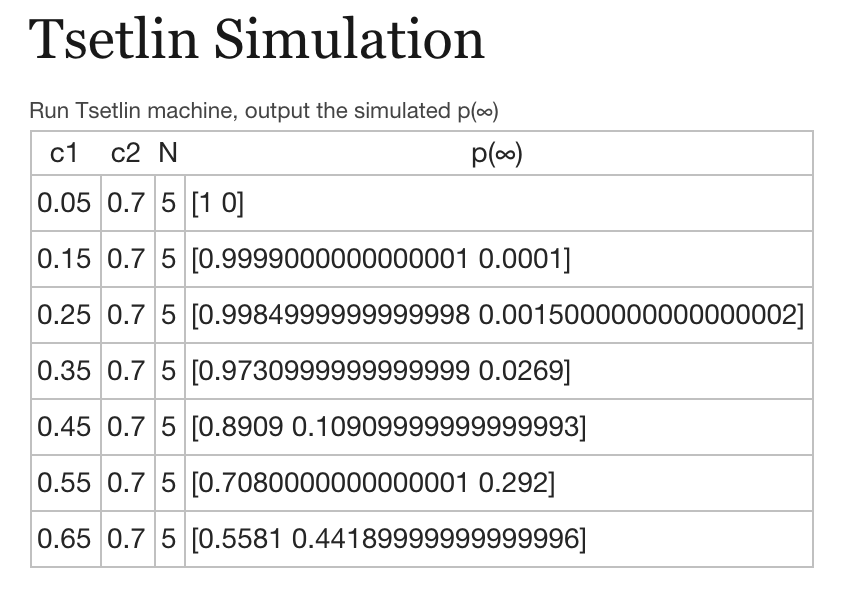
\includegraphics[width=.55\linewidth]{1a}
\end{figure}

\subsection{Min Depth Searching}
Using Binary Search Algorithm to find min N ranging from 1 to 100 that makes the accuracy just greater than 0.95. If the result can not be found, then return the nearest value in the range:

\begin{figure}[H]
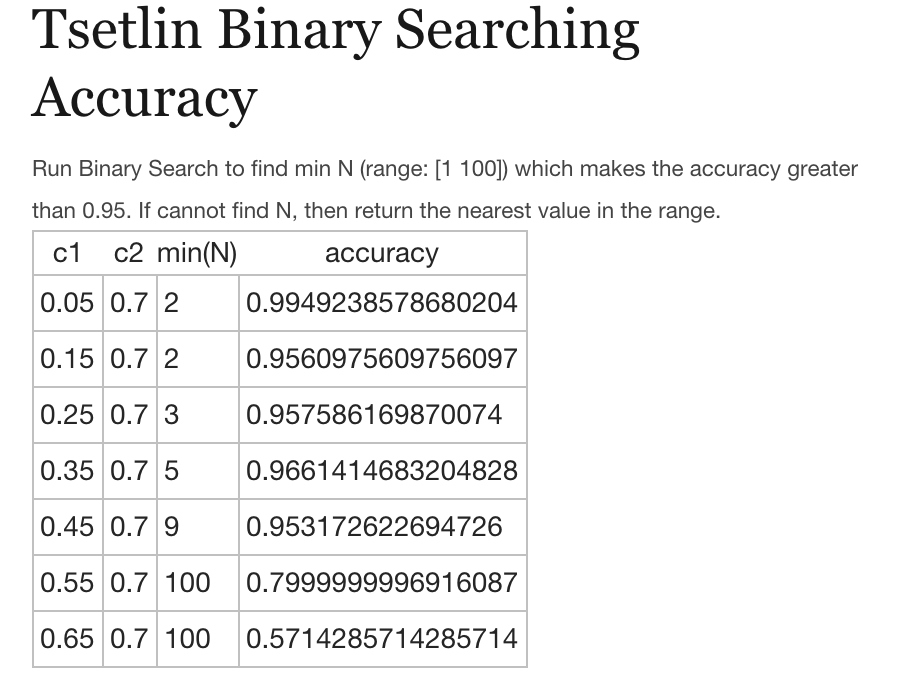
\includegraphics[width=.55\linewidth]{1b}
\end{figure}

\section{Krylov}
Comparing Krylov and Tsetlin with several test cases:

\begin{figure}[H]
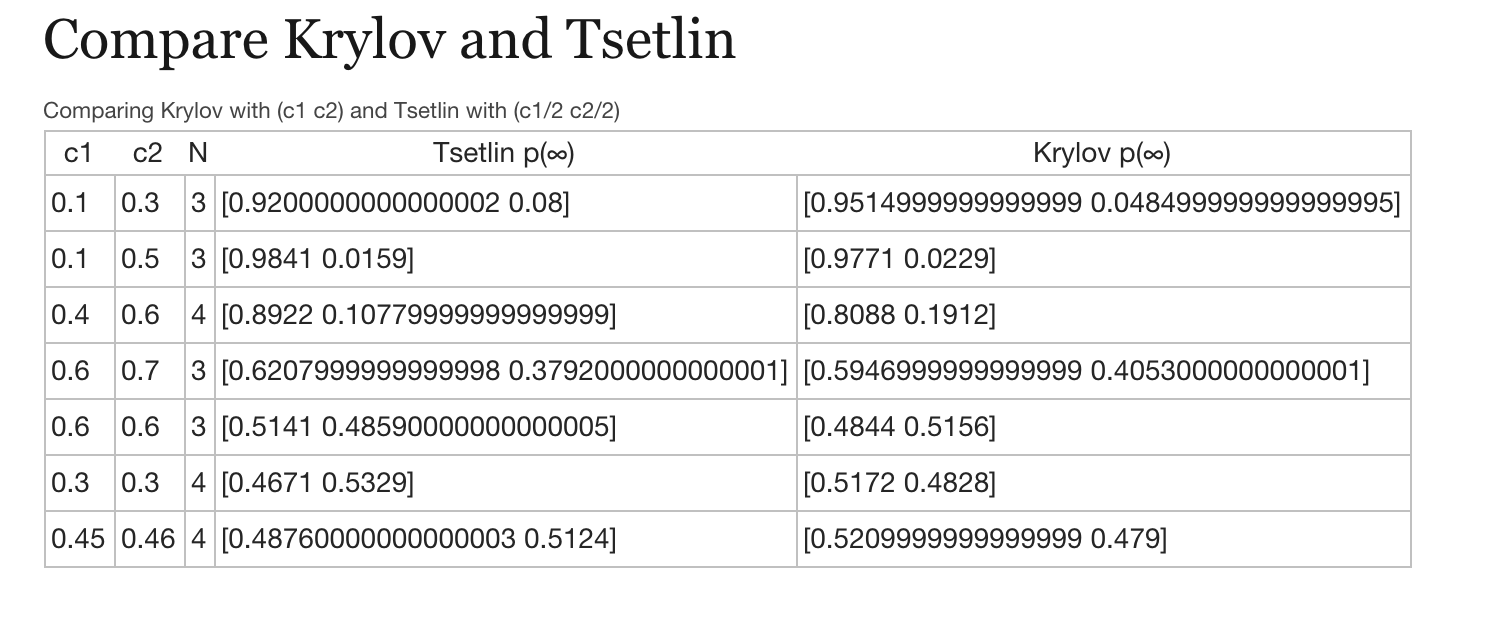
\includegraphics[width=.85\linewidth]{2a}
\end{figure}

\section{$L_{RI}$ Automaton}
\subsection{Simulation}
Run each instance until it is converged ([1 0] or [0 1] state). Here we use $\lambda_{R}=0.8$.

\begin{figure}[H]
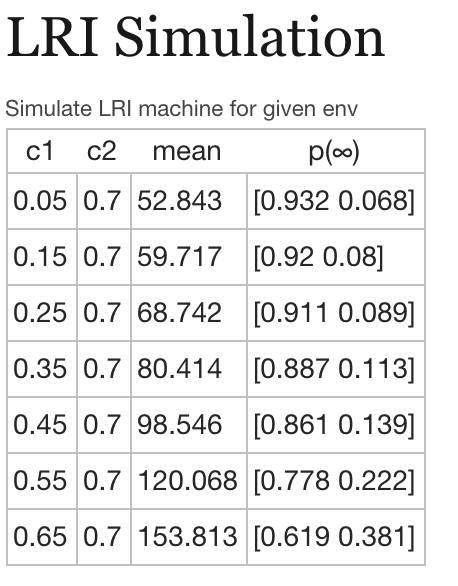
\includegraphics[width=.3\linewidth]{3a}
\end{figure}

From result, when c1 and c2 are more closer to each other, the mean time is larger and accuracy is lower.
\subsection{Search Best $\lambda_{R}$}
Use Binary Search to find the best value $\lambda_{R}$ (which is also minimal) that reaches 0.95 accuracy. For the sake of speed, we only use 200 simulation instances (which also means the precision is 0.005).
Note that this is float number computing, the acceptable accuracy range is $[0.95\text{ } 0.955)$.

\begin{figure}[H]
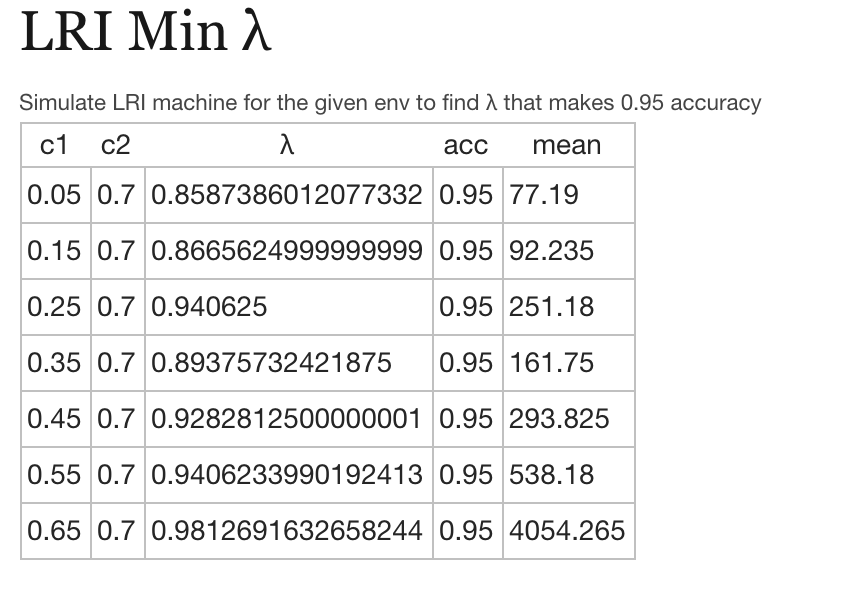
\includegraphics[width=.55\linewidth]{3b}
\end{figure}

\end{document}